\documentclass[openany]{book}
% !TeX TXS-program:compile = txs:///pdflatex/[--shell-escape]
\usepackage{macros}
\usepackage{notes}
\usepackage{animate}
\usepackage{paracol}
\usepackage[dvipsnames]{xcolor}
\usetikzlibrary{shapes.geometric}
\usetikzlibrary{calc}
\usepackage{anyfontsize}

\pgfmathsetmacro{\pendulumswing}{40}
\pgfmathsetmacro{\pendulumlength}{5}

%% PICTURES DIRECTORY %%
\graphicspath{{C:/Users/Michael/Pictures/}}

%% REDEFINING CHAPTER FORMATTING %%
\newif\iftoc\titleformat{\chapter}[display]{\cabin}{}{2in}{
	\raggedleft
	\iftoc
	\vspace{2in}
	\else
	{\LARGE\textsc{Week}~{\cantarell\thechapter}} \\
	\fi
	\Huge\scshape\bfseries
}[\vspace{-20pt}\rule{\textwidth}{0.1pt}\vspace{0.0in}]
\titlespacing{\chapter}{0pt}{
	\iftoc
	-100pt+1in
	\else
	-130pt+1in
	\fi
}{0pt}

%% RENEW TITLE PAGE %%
\renewcommand{\mytitle}[2]{%
	\title{#1}
	\author{Michael Pham}
	\date{#2}
	\maketitle
	\newpage
	\mytoc
	\newpage
}

\begin{document}

\begin{tikzpicture}[remember picture,overlay]
	\fill[BlueViolet] (current page.south west) rectangle (current page.north east);
	
	% Background Hexagon
	\begin{scope}
		\foreach \i in {2.5,...,22}
		{\node[rounded corners,BlueViolet!90,draw,regular polygon,regular polygon sides=6, minimum size=\i cm,ultra thick] at ($(current page.west)+(2.5,-5)$) {} ;}
	\end{scope}
	
	\foreach \i in {0.5,...,22}
	{\node[rounded corners,BlueViolet!90,draw,regular polygon,regular polygon sides=6, minimum size=\i cm,ultra thick] at ($(current page.north west)+(2.5,0)$) {} ;}
	
	\foreach \i in {0.5,...,22}
	{\node[rounded corners,BlueViolet!98,draw,regular polygon,regular polygon sides=6, minimum size=\i cm,ultra thick] at ($(current page.north east)+(0,-9.5)$) {} ;}
	
	\foreach \i in {21,...,6}
	{\node[BlueViolet!95,rounded corners,draw,regular polygon,regular polygon sides=6, minimum size=\i cm,ultra thick] at ($(current page.south east)+(-0.2,-0.45)$) {} ;}
	
	% Course Number
	\node[left,BlueViolet!10,minimum width=0.625*\paperwidth,minimum height=2cm, rounded corners] at ($(current page.north east)+(0,-9.5)$){{\huge Data 100}};
	
	% Title (Line 1)
	\node[left,BlueViolet!5,minimum width=0.625*\paperwidth,minimum height=3cm, rounded corners] at ($(current page.north east)+(0,-11)$){{\fontsize{25}{30} \selectfont \bfseries Principles and Techniques}};
	
	% Title (Line 2)
	\node[left,BlueViolet!5,minimum width=0.625*\paperwidth,minimum height=3cm, rounded corners] at ($(current page.north east)+(0,-12)$){{\fontsize{25}{30} \selectfont \bfseries of Data Science}};
	
	% Name
	\node[left,BlueViolet!5,minimum width=0.625*\paperwidth,minimum height=2cm, rounded corners] at ($(current page.north east)+(0,-14)$){{\Large \textsc{Michael Pham}}};
	
	% Semester	
	\node[rounded corners,fill=BlueViolet!95,text =BlueViolet!5,regular polygon,regular polygon sides=6, minimum size=2.5 cm,inner sep=0,ultra thick] at ($(current page.west)+(2.5,-5)$) {\LARGE \bfseries Sp24};
\end{tikzpicture}

\mytoc

\newpage

\chapter{Introduction to Data Science}
\epigraph{\textit{The purpose of computing is insight,\\not numbers.}}{--- R. Hamming}

\section{Lecture 1 -- 01/16/24}
The course website is located at: \url{https://ds100.org/sp24/}.

\subsection{Course Overview}

\subsubsection{Why Data Science Matters}
Data is used everywhere, from science to sports to medicine. Claims using data also comes up often within discussions (especially about important issues).

Furthermore, Data Science enhances critical thinking. The world is complicated, and decisions are hard. This field fundamentally facilitates decision-making by quantitatively balancing trade-offs.

In order to quantify things reliably, we have to:
\begin{itemize}
	\item Find relevant data;
	\item Recognize the limitations of said data;
	\item Ask the right questions;
	\item Make reasonable assumptions;
	\item Conduct appropriate analysis; and
	\item Synthesize and explain our insights.
\end{itemize}

At each step of this process, we must apply critical thinking and consider how our decisions can affect others.

\newpage

\subsubsection{What is Data Science?}
\begin{defn}[Data Science]\label{def: data science}
	Data Science is the application of data-centric, computational, and inferential thinking to:
	\begin{itemize}
		\item Under the world (science), and
		\item Solve problems (engineering).
	\end{itemize}
\end{defn}

We note that good data analysis is \textbf{not}:
\begin{itemize}
	\item Simple applications of a statistics recipe.
	\item Simple application of software.
\end{itemize}

There are many tools out there for data science, but they are ultimately just tools; we are the ones doing the important thinking.

\subsection{Course Outline}
\subsubsection{Prerequisites}
The official prerequisites are:
\begin{itemize}
	\item \textbf{DATA 8};
	\item \textbf{CS 61A}, DATA C88C, or ENGIN 7; and
	\item EE 16A, \textbf{MATH 54}, or STAT 89A.
\end{itemize}

The bolded course names are the ones that I have already taken.

\subsubsection{Topics (Tentative)}
The tentative list of topics that will be covered in this course is:

\begin{miscbox}{Tentative Topics}
	\begin{multicols}{2}
		\begin{itemize}
			\item Pandas and NumPy
			\item Relational Databases and SQL
			\item Exploratory Data Analysis
			\item Regular Expressions
			\item Visualization
			\begin{itemize}
				\item matplotlib
				\item Seaborn
				\item plotly
			\end{itemize}
			\item Sampling
			\item Probability and random variables
			\item Model design and loss formulation
			\item Linear Regression
			\item Feature Engineering
			\item Regularization, Bias-Variance Tradeoff,\\and Cross-Validation
			\item Gradient Descent
			\item Data Science in the Physical World
			\item Logistic Regression
			\item Clustering
			\item PCA
		\end{itemize}
	\end{multicols}
\end{miscbox}

\subsubsection{Course Components}
With respect to lectures and assignments, the course is structured as follows:
\begin{miscbox}{Course Components}
	\centering
	\begin{center}
		\begin{tabularx}{\textwidth}{Y|Y|Y|Y|Y}
			\textbf{Mo} & \textbf{Tu} & \textbf{We} & \textbf{Th} & \textbf{Fr} \\
			\hline
			& \color{darkgreen}{Live Lecture} & & \color{darkgreen}{Live Lecture} & \\
			\hline
			& \color{darkblue}{Discussion} & \color{darkblue}{Discussion} & & \\
			\hline
			& \color{darkgray}{Office Hours} & \color{darkgray}{Office Hours} & \color{darkgray}{Office Hours} & \color{darkgray}{Office Hours} \\
			\hline
			& & & \color{red}{\textbf{Homework N-1 due}} & \color{darkred}{Homework N released} \\
			\hline
			& \color{red}{\textbf{Lab N-1 due}} & & & \color{darkred}{Lab N released}
		\end{tabularx}
	\end{center}
\end{miscbox}

For lectures, note that there attendance is mandatory; participation will be graded on a 0/1 basis:
\begin{itemize}
	\item Synchronous Participation: complete at least one participation poll question during the live lecture timeslot (11:00am-12:30pm, Tuesdays and Thursdays). As long as you submit a response to at least one poll question in this timeframe, you will receive synchronous attendance credit.
	\item Asynchronous Participation: complete all participation poll questions from the link provided on the course website within one week of the corresponding lecture.
	\item In both cases, participation is graded on completion, not correctness.
\end{itemize}

Also, if we submit all participation polls over the semester, there will be a 0.5\% bonus points applied to the final overall grade.

\subsubsection{Grading}
The grading scheme for this class is as follows:
\begin{miscbox}{Grading Scheme}
	\begin{center}
		\begin{tabularx}{6cm}{X|c}
			\textbf{Category} & \\
			\hline
			Homeworks & 25\% \\
			\hline
			Projects & 10\% \\
			\hline
			Labs & 5\% \\
			\hline
			Discussions & -\\
			\hline
			Lecture Participation & 5\% \\
			\hline
			Midterm Exam & 22.5\% \\
			\hline
			Final Exam & 32.5\% \\
		\end{tabularx}
	\end{center}
\end{miscbox}

\begin{warn}
	\textbf{Important}:
	\begin{itemize}
		\item Midterm: Thursday, March 7, 7-9 PM PST.
		\item Final: Thursday, May 9, 8-11 AM PST.
	\end{itemize}
\end{warn}

\subsection{The Data Science Lifecycle}
The data science lifecycle is a high-level description of the data science workflow. Note in the diagram below that there are two distinct entry points.

\begin{center}
	\begin{animateinline}[controls={play, stop}, controlsaligned = center, loop]{1}
		\multiframe{5}{}{
			% FRAME 1 %
			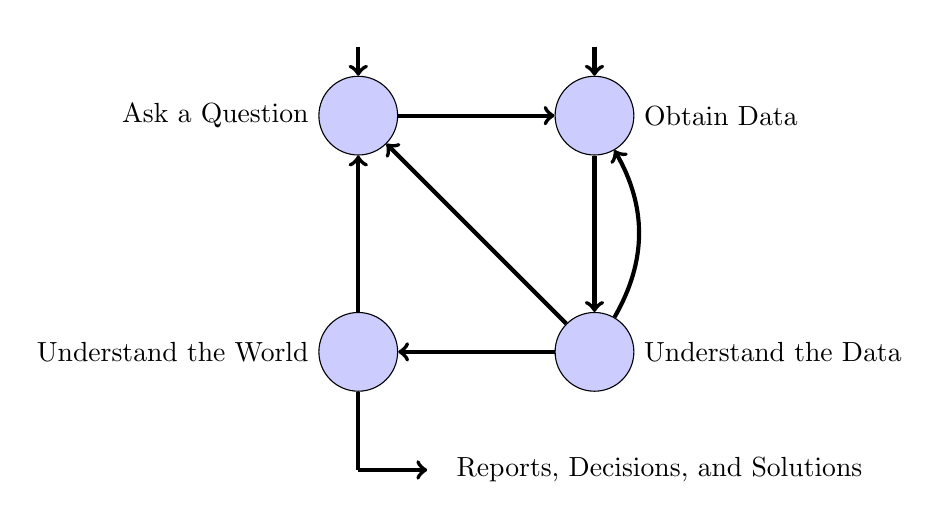
\begin{tikzpicture}
				\node[circle, draw, inner sep = 0pt, minimum width = 1cm, fill = blue!20] at (0,0) (understand_world) {};
				\node[circle, draw, inner sep = 0pt, minimum width = 1cm, fill = blue!20] at (0,3) (ask) {};s
				\node[circle, draw, inner sep = 0pt, minimum width = 1cm, fill = blue!20] at (3,3) (obtain) {};
				\node[circle, draw, inner sep = 0pt, minimum width = 1cm, fill = blue!20] at (3,0) (understand_data) {};
				
				\node at (0,4) (topask) {};
				\node at (3,4) (topobtain) {};
				
				\node at (0,-1.5) (ghostnode) {};
				\node at (1,-1.5) (report) {};
				
				\node[left] at (ask.west){Ask a Question};
				\node[left] at (understand_world.west){Understand the World};
				\node[right] at (obtain.east){Obtain Data};
				\node[right] at (understand_data.east){Understand the Data};
				\node[right] at (report.east){Reports, Decisions, and Solutions};
				
				\draw (understand_world) edge [->, line width = 1.5pt] (ask);
				\draw (understand_data) edge [->, line width = 1.5pt] (understand_world);
				\draw (understand_data) edge [->, line width = 1.5pt] (ask);
				\draw (ask) edge [->, line width = 1.5pt] (obtain);
				\draw (obtain) edge [->, line width = 1.5pt] (understand_data);
				\draw (understand_data) edge[bend right, ->, line width = 1.5pt] node [left] {} (obtain);
				
				\draw (topask) edge [->, line width = 1.5pt] (ask);
				\draw (topobtain) edge [->, line width = 1.5pt] (obtain);
				
				\draw (understand_world) edge [line width = 1.5pt] (ghostnode.center);
				\draw (ghostnode.center) edge [->, line width = 1.5pt] (report);
			\end{tikzpicture}
		
			\newframe
			% FRAME 2 %
			\begin{tikzpicture}
				\node[circle, draw, inner sep = 0pt, minimum width = 1cm, fill = blue!20, opacity = 0.25] at (0,0) (understand_world) {};
				\node[circle, draw, inner sep = 0pt, minimum width = 1cm, fill = blue!20] at (0,3) (ask) {};s
				\node[circle, draw, inner sep = 0pt, minimum width = 1cm, fill = blue!20, opacity = 0.25] at (3,3) (obtain) {};
				\node[circle, draw, inner sep = 0pt, minimum width = 1cm, fill = blue!20, opacity = 0.25] at (3,0) (understand_data) {};
				
				\node at (0,4) (topask) {};
				\node at (3,4) (topobtain) {};
				
				\node at (0,-1.5) (ghostnode) {};
				\node at (1,-1.5) (report) {};
				
				\node[left] at (ask.west){\color{darkblue}{\textbf{Ask a Question}}};
				\node[left, opacity = 0.25] at (understand_world.west){Understand the World};
				\node[right, opacity = 0.25] at (obtain.east){Obtain Data};
				\node[right, opacity = 0.25] at (understand_data.east){Understand the Data};
				\node[right, opacity = 0.25] at (report.east){Reports, Decisions, and Solutions};
				
				\draw (understand_world) edge [->, line width = 1.5pt] (ask);
				\draw (understand_data) edge [->, line width = 1.5pt, opacity = 0.25] (understand_world);
				\draw (understand_data) edge [->, line width = 1.5pt] (ask);
				\draw (ask) edge [->, line width = 1.5pt] (obtain);
				\draw (obtain) edge [->, line width = 1.5pt, opacity = 0.25] (understand_data);
				\draw (understand_data) edge[bend right, ->, line width = 1.5pt, opacity = 0.25] node [left] {} (obtain);
				
				\draw (topask) edge [->, line width = 1.5pt] (ask);
				\draw (topobtain) edge [->, line width = 1.5pt, opacity = 0.25] (obtain);
				
				\draw (understand_world) edge [line width = 1.5pt, opacity = 0.25] (ghostnode.center);
				\draw (ghostnode.center) edge [->, line width = 1.5pt, opacity = 0.25] (report);
			\end{tikzpicture}
		
			\newframe
			% FRAME 3 %
			\begin{tikzpicture}
				\node[circle, draw, inner sep = 0pt, minimum width = 1cm, fill = blue!20, opacity = 0.25] at (0,0) (understand_world) {};
				\node[circle, draw, inner sep = 0pt, minimum width = 1cm, fill = blue!20, opacity = 0.25] at (0,3) (ask) {};s
				\node[circle, draw, inner sep = 0pt, minimum width = 1cm, fill = blue!20] at (3,3) (obtain) {};
				\node[circle, draw, inner sep = 0pt, minimum width = 1cm, fill = blue!20, opacity = 0.25] at (3,0) (understand_data) {};
				
				\node at (0,4) (topask) {};
				\node at (3,4) (topobtain) {};
				
				\node at (0,-1.5) (ghostnode) {};
				\node at (1,-1.5) (report) {};
				
				\node[left, opacity = 0.25] at (ask.west){Ask a Question};
				\node[left, opacity = 0.25] at (understand_world.west){Understand the World};
				\node[right] at (obtain.east){\color{darkblue}{\textbf{Obtain Data}}};
				\node[right, opacity = 0.25] at (understand_data.east){Understand the Data};
				\node[right, opacity = 0.25] at (report.east){Reports, Decisions, and Solutions};
				
				\draw (understand_world) edge [->, line width = 1.5pt, opacity = 0.25] (ask);
				\draw (understand_data) edge [->, line width = 1.5pt, opacity = 0.25] (understand_world);
				\draw (understand_data) edge [->, line width = 1.5pt, opacity = 0.25] (ask);
				\draw (ask) edge [->, line width = 1.5pt] (obtain);
				\draw (obtain) edge [->, line width = 1.5pt] (understand_data);
				\draw (understand_data) edge[bend right, ->, line width = 1.5pt] node [left] {} (obtain);
				
				\draw (topask) edge [->, line width = 1.5pt, opacity = 0.25] (ask);
				\draw (topobtain) edge [->, line width = 1.5pt] (obtain);
				
				\draw (understand_world) edge [line width = 1.5pt, opacity = 0.25] (ghostnode.center);
				\draw (ghostnode.center) edge [->, line width = 1.5pt, opacity = 0.25] (report);
			\end{tikzpicture}
		
			\newframe
			% FRAME 4 %
			\begin{tikzpicture}
				\node[circle, draw, inner sep = 0pt, minimum width = 1cm, fill = blue!20, opacity = 0.25] at (0,0) (understand_world) {};
				\node[circle, draw, inner sep = 0pt, minimum width = 1cm, fill = blue!20, opacity = 0.25] at (0,3) (ask) {};s
				\node[circle, draw, inner sep = 0pt, minimum width = 1cm, fill = blue!20, opacity = 0.25] at (3,3) (obtain) {};
				\node[circle, draw, inner sep = 0pt, minimum width = 1cm, fill = blue!20] at (3,0) (understand_data) {};
				
				\node at (0,4) (topask) {};
				\node at (3,4) (topobtain) {};
				
				\node at (0,-1.5) (ghostnode) {};
				\node at (1,-1.5) (report) {};
				
				\node[left, opacity = 0.25] at (ask.west){Ask a Question};
				\node[left, opacity = 0.25] at (understand_world.west){Understand the World};
				\node[right, opacity = 0.25] at (obtain.east){Obtain Data};
				\node[right] at (understand_data.east){\color{darkblue}{\textbf{Understand the Data}}};
				\node[right, opacity = 0.25] at (report.east){Reports, Decisions, and Solutions};
				
				\draw (understand_world) edge [->, line width = 1.5pt, opacity = 0.25] (ask);
				\draw (understand_data) edge [->, line width = 1.5pt] (understand_world);
				\draw (understand_data) edge [->, line width = 1.5pt] (ask);
				\draw (ask) edge [->, line width = 1.5pt, opacity = 0.25] (obtain);
				\draw (obtain) edge [->, line width = 1.5pt] (understand_data);
				\draw (understand_data) edge[bend right, ->, line width = 1.5pt] node [left] {} (obtain);
				
				\draw (topask) edge [->, line width = 1.5pt, opacity = 0.25] (ask);
				\draw (topobtain) edge [->, line width = 1.5pt, opacity = 0.25] (obtain);
				
				\draw (understand_world) edge [line width = 1.5pt, opacity = 0.25] (ghostnode.center);
				\draw (ghostnode.center) edge [->, line width = 1.5pt, opacity = 0.25] (report);
			\end{tikzpicture}
		
			\newframe
			% FRAME 5 %
			\begin{tikzpicture}
				\node[circle, draw, inner sep = 0pt, minimum width = 1cm, fill = blue!20] at (0,0) (understand_world) {};
				\node[circle, draw, inner sep = 0pt, minimum width = 1cm, fill = blue!20, opacity = 0.25] at (0,3) (ask) {};s
				\node[circle, draw, inner sep = 0pt, minimum width = 1cm, fill = blue!20, opacity = 0.25] at (3,3) (obtain) {};
				\node[circle, draw, inner sep = 0pt, minimum width = 1cm, fill = blue!20, opacity = 0.25] at (3,0) (understand_data) {};
				
				\node at (0,4) (topask) {};
				\node at (3,4) (topobtain) {};
				
				\node at (0,-1.5) (ghostnode) {};
				\node at (1,-1.5) (report) {};
				
				\node[left, opacity = 0.25] at (ask.west){Ask a Question};
				\node[left] at (understand_world.west){\color{darkblue}{\textbf{Understand the World}}};
				\node[right, opacity = 0.25] at (obtain.east){Obtain Data};
				\node[right, opacity = 0.25] at (understand_data.east){Understand the Data};
				\node[right] at (report.east){Reports, Decisions, and Solutions};
				
				\draw (understand_world) edge [->, line width = 1.5pt] (ask);
				\draw (understand_data) edge [->, line width = 1.5pt] (understand_world);
				\draw (understand_data) edge [->, line width = 1.5pt, opacity = 0.25] (ask);
				\draw (ask) edge [->, line width = 1.5pt, opacity = 0.25] (obtain);
				\draw (obtain) edge [->, line width = 1.5pt, opacity = 0.25] (understand_data);
				\draw (understand_data) edge[bend right, ->, line width = 1.5pt, opacity = 0.25] node [left] {} (obtain);
				
				\draw (topask) edge [->, line width = 1.5pt, opacity = 0.25] (ask);
				\draw (topobtain) edge [->, line width = 1.5pt, opacity = 0.25] (obtain);
				
				\draw (understand_world) edge [line width = 1.5pt] (ghostnode.center);
				\draw (ghostnode.center) edge [->, line width = 1.5pt] (report);
			\end{tikzpicture}
		}
	\end{animateinline}
\end{center}

The Data Science Lifecycle goes as follows:
\begin{enumerate}
	\item \textbf{Question/Problem Formulation}
	\begin{itemize}
		\item What do we want to know?
		\item What problems are we trying to solve?
		\item What hypotheses do we want to test?
		\item What are our metrics for success?
	\end{itemize}
	\item \textbf{Data Acquisition and Cleaning}
	\begin{itemize}
		\item What data do we have and what data do we need?
		\item How will we sample more data?
		\item Is our data representative of the population we want to study?
	\end{itemize}
	\item \textbf{Exploratory Data Analysis and Visualization}
	\begin{itemize}
		\item How is our data organized, and what does it contain?
		\item Do we already have the relevant data?
		\item What are the biases, anomalies, or other issues with the data?
		\item How do we transform the data to enable effective analysis?
	\end{itemize}
	\item \textbf{Prediction and Inference}
	\begin{itemize}
		\item What does the data say about the world?
		\item Does it answer our questions or accurately solve the problem?
		\item How robust are our conclusions and can we trust the predictions?
	\end{itemize}
\end{enumerate}

\section{Lecture 2 -- 01/18/24}
\subsection{Tabular Data}
Tabular data simply refers to data that is in a table, where each row represents one observation and each column representing some characteristic, or feature, of the observation.

In this class, we will be using the Python \mylib{\texttt{pandas}} library.
\begin{figurebox}{\texttt{pandas} logo.}
	\centering\includegraphics[height = 2cm]{pandas.png}
\end{figurebox}

With Pandas, we can accomplish a lot of things. Below are a list of some things we will be learning to use Pandas for in this course:
\begin{itemize}
	\item Arranging data in a tabular format.
	\item Extract useful information filtered by specific conditions.
	\item Operate on data to gain new insights.
	\item Apply \mylib{\texttt{NumPy}} functions to our data.
	\item Perform vectorized computations to speed up our analysis.
\end{itemize}

\subsection{DataFrames and Series}
\begin{defn}[DataFrames]\label{def: DataFrames}
	In the language of \texttt{pandas}, we refer to a table as a \texttt{DataFrame}, which is a collection of named columns called \texttt{Series}.
\end{defn}

\begin{defn}[Series]\label{def: Series}
	A \texttt{Series} is a one-dimensional array-like object. It contains:
	\begin{itemize}
		\item A sequence of \texttt{values} of the same type.
		\item A sequence of data labels, called the index.
	\end{itemize}
\end{defn}

\subsubsection{The Series Object}
First, we look at some basic details about the \texttt{Series} object.

\begin{code}{python}{\texttt{Series} Basics}
import pandas as pd

# Creating a Series object
s = pd.Series(["Welcome", "to", "data 100"])
s.index # RangeIndex(start=0, stop=3, step=1)
s.values # array(['welcome', 'to', 'data 100'], dtype='object')
\end{code}

We see that the \texttt{Series} object has \texttt{index} and \texttt{values} variables. Note that we can in fact set custom indices, as shown below:

\begin{code}{python}{Custom Indexing}
# Creating Series with custom indexing
s = pd.Series([-1, 10, 2], index = ["a", "b", "c"])
s.index # Index(['a', 'b', 'c'], dtype='object')

# Changing Series' index
s.index = ["first", "second", "third"]
s.index # Index(['first', 'second', 'third'], dtype='object')
\end{code}

Finally, we can also select a single value or a set of values in a \texttt{Series} object using:
\begin{itemize}
	\item A single label.
	\item A list of labels.
	\item A filtering condition.
\end{itemize}

\begin{code}{python}{Selection}
# Creating a Series
s = pd.Series([4, -2, 0, 6], index = ["a", "b", "c", "d"])

# Selection
s["a"] # Single Label: [4]
s[["a", "c"]] # List of Labels: [4, 0]
s[s > 0] # Filtering Condition: [4, 6]
\end{code}

Note that for selection via filtering condition, we do the following:
\begin{enumerate}
	\item Apply a boolean condition to the \texttt{Series} that satisfy a particular condition.
	\item Index into our \texttt{Series} using this boolean condition. \texttt{pandas} will select only the entries in the \texttt{Series} that satisfy the condition.
\end{enumerate}

\subsubsection{DataFrames}
Typically, we imagine \texttt{Series} as columns within a \texttt{DataFrame} object.

One way to think of a \texttt{DataFrame} is a collection of \texttt{Series} object which shares the same index.

\begin{figurebox}{Relation between \texttt{DataFrame} and \texttt{Series}}
	\centering\includegraphics[height=3.5cm]{dataframe1.png}
\end{figurebox}

The syntax for creating a \texttt{DataFrame} is \inlinecode{\mintinline{python}{pandas.DataFrame(data, index, columns)}}.

We have many approaches for creating a \texttt{DataFrame}. Below are some of the most common ones:
\begin{itemize}
	\item From a CSV file.
	\item Using a list and column name(s).
	\item From a dictionary.
	\item From a \texttt{Series}.
\end{itemize}

\begin{code}{python}{Creating \texttt{DataFrame} Objects}
# From a CSV File
elections = pd.read_csv("data/elections.csv")

# We can also create a DataFrame with one of the columns as the index value
elections = pd.read_csv("data/elections.csv", index_col="Year")

# From a list and column name(s)
pd.DataFrame([1, 2, 3], columns=["Numbers"]) # One column
pd.DataFrame([[1, "one"], [2, "two"]], columns = ["Number", "Description"]) # Multiple columns

# From a dictionary
pd.DataFrame({"Fruit":["Strawberry", "Orange"], "Price": [5.49, 3.99]}) # Specify columns of the DataFrame
pd.DataFrame([{"Fruit":"Strawberry", "Price":5.49}, {"Fruit":"Orange", "Price":3.99}]) # Specify the rows of the DataFrame

# From a Series
s_a = pd.Series(["a1", "a2", "a3"], index = ["r1", "r2", "r3"])
s_b = pd.Series(["b1", "b2", "b3"], index = ["r1", "r2", "r3"])

pd.DataFrame({"A-column":s_a, "B-column":s_b})
\end{code}

\begin{warn}
	Note that indices are not necessarily row numbers! We can set non-numeric values to be the index as well. Furthermore, they aren't necessarily unique either; we can have duplicate values in the index. 
\end{warn}

For example, suppose we ran the following code: 

\begin{center}
	\inlinecode{\mintinline{python}{elections = pd.read_csv("data/elections.csv", index_col = "Candidate")}}
\end{center}

Then, we will get the following \texttt{DataFrame}:
\begin{figurebox}{\texttt{DataFrame} with non-numeric, non-unique indexing.}
	\centering\includegraphics[scale=0.5]{dataframe2}
\end{figurebox}

After creating a \texttt{DataFrame}, we can then change its index using \inlinecode{\mintinline{python}{df.set_index(column_name)}}. And if we happen to change our mind, we can simply do \inlinecode{\mintinline{python}{df.reset_index()}}.

However, while indexes are not necessarily unique, column names in \texttt{pandas} are almost always unique. Having two columns share a name is also just bad practice in general.

We can also extract basic, useful information about a \texttt{DataFrame}, such as its index, columns, and shape.

\begin{code}{python}{Getting Basic \texttt{DataFrame} Information}
# Getting the row labels
elections.index

# Getting the column labels
elections.columns

# Getting the shape of the DataFrame, given in the form (row, col)
elections.shape
\end{code}

\subsection{Data Extraction}
When dealing with data, we want to be able to extract information that we want to work with specifically. Common ways we may want our data is as follows:
\begin{itemize}
	\item Grab the first or last \texttt{n} rows in the \texttt{DataFrame}.
	\item Grab data with a certain label.
	\item Grab data at a certain position. 
\end{itemize}

\subsubsection{.head and .tail}
The simplest scenarios: We want to extract the first or last \texttt{n} rows from the \texttt{DataFrame}.
\begin{itemize}
	\item \inlinecode{\mintinline{python}{df.head(n)}} will return the first \texttt{n} rows of the DataFrame \texttt{df}.
	\item \inlinecode{\mintinline{python}{df.tail(n)}} will return the last \texttt{n} rows.
\end{itemize}

\subsubsection{Label-based Extraction (.loc)}
Something more complex is extracting data with specific columns or index labels. One way to do this is with \inlinecode{\mintinline{python}{.loc}}, which has the following format:
\begin{center}
	\inlinecode{\mintinline{python}{df.loc[row_labels, column_labels]}}
\end{center}

The \inlinecode{\mintinline{python}{.loc}} accessor lets us specify the labels of rows/columns we want to extract. These are the bolded values in a DataFrame.

Arguments to \inlinecode{\mintinline{python}{.loc}} can be:
\begin{itemize}
	\item A list.
	\item A slice.
	\item A single value.
\end{itemize}
\begin{warn}
	Note that for \inlinecode{\mintinline{python}{.loc}}, the slice is, unlike normal Python syntax, \textbf{inclusive} of the right side.
\end{warn}

\begin{code}{python}{Extraction with \texttt{.loc}}
	# Using a list
	elections.loc[[87, 25, 179], ["Year", "Candidate", "Result"]]
	
	# Using a slice
	elections.loc[[87, 25, 179], "Popular vote":"%"]
	elections.loc[:, ["Year", "Candidate", "Result"]] # Gets all rows
	elections.loc[[87, 25, 179], :] # Gets all columns
	
	# Using a single value.
	elections.loc[[87, 25, 179], "Popular vote"] # Note that this returns the Popular vote series, with only the select indices
	elections.loc[0, "Candidate"] # This returns the string value at index 0 from the Candidate column
\end{code}

\begin{figurebox}{\texttt{.loc} using a list.}
	\centering\includegraphics[scale=0.75]{dataframe3}
\end{figurebox}

\begin{figurebox}{\texttt{.loc} using a slice.}
	\centering\includegraphics[scale=0.75]{dataframe4}
\end{figurebox}

\subsubsection{Integer-based Extraction (.iloc)}
A different scenario: We want to extract data according to its position.

To do this, we use \inlinecode{\mintinline{python}{.iloc}}, which allows us to specify the integers of rows and columns we wish to extract. It has the following format:
\begin{center}
	\inlinecode{\mintinline{python}{df.iloc[row_integers, column_integers]}}
\end{center}

Arguments to \inlinecode{\mintinline{python}{.iloc}} can be:
\begin{itemize}
	\item A list.
	\item A slice.
	\item A single value.
\end{itemize}
\begin{warn}
	Note that while the slice was \textbf{inclusive} of the right side for \inlinecode{\mintinline{python}{.loc}}, it is \textbf{exclusive} for \inlinecode{\mintinline{python}{.iloc}}...! Very confusing!!
\end{warn}

The syntax for \inlinecode{\mintinline{python}{.iloc}} is identical to \inlinecode{\mintinline{python}{.loc}}.

\subsubsection{.loc versus .iloc}
While \inlinecode{\mintinline{python}{.loc}} is both safer (i.e. if the order of the data gets shuffled around, our code will still work) and more readable (people actually know what columns we want), \inlinecode{\mintinline{python}{.iloc}} can still be useful!

\begin{example}[Using \texttt{.iloc}]
	If we have a \texttt{DataFrame} of movie earnings sorted by earnings, we can use \inlinecode{\mintinline{python}{.iloc}} to get the median earnings for a given year by indexing into the middle.
\end{example}

\subsubsection{Context-dependent Extraction ([])}
Finally, we have the possibly most-complicated way of extracting data: context-dependent extraction.

\texttt{[]} only takes one argument, which may be:
\begin{itemize}
	\item A slice of row integers.
	\item A list of column labels.
	\item A single column label.
\end{itemize}

\begin{code}{python}{Extraction with \texttt{[]}}
# Using a slice of row integers
elections[3:7]

# Using a list of column labels
elections[["Year", "Candidate", "Result"]]

# Using a single column label
elections["Candidate"]
\end{code}

Using \texttt{[]} is a lot more concise than either \texttt{.loc} or \texttt{.iloc}, hence it's often used more in practice than the other extraction methods.

\chapter{Pandas, and more Pandas!}
\epigraph{\textit{You're as soft as Po,\\the Kung Fu Panda!}}{--- Z. Sherwin}

\section{Lecture 3 -- 01/23/24}
\subsection{Conditional Selection}
We can extract rows that satisfy a given condition. Note that \inlinecode{\mintinline{python}{.loc}} and \texttt{[]} also accept boolean arrays as input; using this, only rows that correspond to \texttt{True} will be extracted.

For example, consider the following code:
\begin{code}{python}{Conditional Selection}
# Getting first ten rows
babynames_first_10_rows = babynames.loc[:9, :]

# Selection with []
babynames_first_10_rows[[True, False, True, False, True, False, True, False, True, False]]

# Selection with .loc
babynames_first_10_rows.loc[[True, False, True, False, True, False, True, False, True, False], :]
\end{code}

In both cases, the following DataFrame will be returned:
\begin{figurebox}{\texttt{DataFrame} with filtered rows.}
	\centering\includegraphics[scale=0.5]{dataframe5}
\end{figurebox}

Using this, we can then extend it to more powerful conditional selections; for example, we can select only rows that are female, \textit{or} were born before 2000 in the DataFrame (or both!):
\begin{center}
	\inlinecode{\mintinline{python}{babynames[(babynames["Sex"] == "F") | (babynames["Year"] < 2000)]}}
\end{center}

This example above also shows us how we can use bitwise operators with our conditionals.

\begin{miscbox}{Bitwise Operators}
	If $p$ and $q$ are boolean arrays or \texttt{Series}, then:
	\begin{center}
		\begin{tabularx}{\textwidth}{|Y|Y|Y|}
			\hline
			\textbf{Symbol} & \textbf{Usage} & \textbf{Meaning} \\
			\hline
			$\sim$ & $\sim p$ & Negation of $p$ \\
			\hline
			$\mid$ & $p \mid q$ & $p$ or $q$ \\
			\hline
			$\&$ & $p \mathbin{\&} q$ & $p$ and $q$ \\
			\hline
			$\mathbin{\char`\^}$ & $p \mathbin{\char`\^} q$ & $p$ xor $q$ \\
			\hline
		\end{tabularx}
	\end{center}
\end{miscbox}

While boolean array selection is useful, it can make our code overly verbose for more complicated conditions. Luckily, \texttt{pandas} offers many alternatives:
\begin{itemize}
	\item \inlinecode{\mintinline{python}{.isin}}
	\item \inlinecode{\mintinline{python}{.str.startswith}}
	\item \inlinecode{\mintinline{python}{.groupby.filter}}
\end{itemize}

\begin{code}{python}{Using \texttt{.isin}}
names = ["Bella", "Alex", "Narges", "Lisa"]

# .isin
babynames[babynames["Name"].isin(names)] # Returns a Series whose entry is True if the corresponding name in babynames is found in the names list

# .str.startswith
babynames[babynames["Name"].str.startswith("N")] # Returns a Series whose entry is True if the corresponding name starts with N
\end{code}

\subsection{Adding, Removing, and Modifying Columns}
\subsubsection{Adding and Modifying Columns}
To add a column, we proceed as follows:
\begin{enumerate}
	\item Use \texttt{[]} to reference the desired new column.
	\item Assign this column to a Series or array of the appropriate length.
\end{enumerate}

We can also modify a column's name or values. The latter's steps are similar to adding a column. For the former, we can use the \inlinecode{\mintinline{python}{.rename()}} function which takes in a dictionary mapping old column names to the new one.

Below, we show how to add, then modify a column:

\begin{code}{python}{Adding and Modifying Columns}
# Create a Series of the length of each name
babyname_lengths = babynames["Name"].str.len()

# Add a column named "name_lengths" that includes the length of each name
babynames["name_lengths"] = babyname_lengths

# Modify the "name_lengths" column to be one less than its original value
babynames["name_lengths"] = babynames["name_lengths"]-1

# Rename "name_lengths" to "Length"
babynames = babynames.rename(columns={"name_lengths":"Length"})
\end{code}

\subsubsection{Removing Columns}
Removing columns a bit more tricky. First, if we want to drop a column, we can use \inlinecode{\mintinline{python}{.drop()}}.

\begin{warn}
	Note that \inlinecode{\mintinline{python}{.drop()}} assumes that we're dropping a row by default; to drop columns, we have to use \inlinecode{\mintinline{python}{axis = "columns"}}...!
	
	Furthermore, we \textbf{must} reassign to the updated DataFrame after dropping a row/column. By default, \texttt{pandas} methods create a copy of the DataFrame, without changing the original DataFrame at all. To apply our changes, we must update our DataFrame to this new, modified copy.
\end{warn}

\begin{code}{python}{Removing Columns}
# Does NOT modify babynames DataFrame
babynames.drop("Length", axis="columns")

# Does modify babynames (through reassignment)
babynames = babynames.drop("Length", axis="columns")
\end{code}

\subsection{Useful Utility Functions}
As stated previously, one of the libraries which we will use is \texttt{NumPy}, which has a lot of useful operations such as \inlinecode{\mintinline{python}{np.mean()}} and \inlinecode{\mintinline{python}{np.max()}}.

And with the \texttt{pandas} library, we have access to a wider array of useful functions. Some which will be covered in this lecture are:
\begin{itemize}
	\item \inlinecode{\mintinline{python}{.shape}}: returns the shape of a \texttt{DataFrame} or \texttt{Series} in the form (rows, cols).
	\item \inlinecode{\mintinline{python}{.size}}: returns the total number of entries in a \texttt{DataFrame} or \texttt{Series}.
	\item \inlinecode{\mintinline{python}{.describe()}}: returns a ``description" of a \texttt{DataFrame} or \texttt{Series} that lists summary statistics of the data.
	\begin{itemize}
		\item For \texttt{DataFrame}: count, mean, std, min/max, quartiles.
		\item For \texttt{Series}: count, unique, top, freq
	\end{itemize}
	\item \inlinecode{\mintinline{python}{.sample()}}: samples a random selection of rows from a \texttt{DataFrame}.
	\begin{itemize}
		\item By default, it is without replacement. Use \inlinecode{\mintinline{python}{replace=True}} for replacement.
		\item Naturally, can be chained with other methods and operators.
	\end{itemize}
	\item \inlinecode{\mintinline{python}{.value_counts()}}: counts the number of occurrences of each unique value in a \texttt{Series}.
	\item \inlinecode{\mintinline{python}{.unique()}}: returns an array of every unique value in a \texttt{Series}.
	\item \inlinecode{\mintinline{python}{.sort_values()}}: sort a \texttt{DataFrame} (or \texttt{Series}).
	\begin{itemize}
		\item \inlinecode{\mintinline{python}{Series.sort_values()}} will automatically sort all values in the \texttt{Series}.
		\item \inlinecode{\mintinline{python}{DataFrame.sort_values(column_name)}} must specify the name of the column to be used for sorting.
	\end{itemize}
\end{itemize}
\begin{warn}
	Note that for \inlinecode{\mintinline{python}{.sort_values()}}, rows are sorted in ascending order.
	
	We can do \inlinecode{\mintinline{python}{.sort_values(ascending=False)}} to sort in descending order.
\end{warn}

\subsubsection{Custom Sorting}
Suppose that we wanted to sort using some custom sorting system. To accomplish this task, there are three main ways of doing so:
\begin{enumerate}
	\item Creating a temporary column and sort Based on the new column.
	\item Sorting using the \texttt{key} argument.
	\item Sorting using the \texttt{map} function.
\end{enumerate}
\begin{code}{python}{Custom Sorting}
# Create a Series of the length of each name
babyname_lengths = babynames["Name"].str.len()

# Approach 1: Create a temporary column
babynames["name_lengths"] = babyname_lengths # Add a column named "name_lengths" that includes the length of each name
babynames = babynames.sort_values(by="name_lengths", ascending=False)

# Approach 2: Sorting using the key Argument
babynames.sort_values("Name", key=lambda x: x.str.len(), ascending=False)

# Approach 3: Sorting using the map Function
def dr_ea_count(string):
  return string.count('dr') + string.count('ea')

babynames["dr_ea_count"] = babynames["Name"].map(dr_ea_count) # Use map to apply dr_ea_count to each name in the "Name" column
babynames = babynames.sort_values(by="dr_ea_count", ascending=False)
\end{code}

\section{Lecture 4 -- 01/25/24}
\subsection{Grouping}
Our goal:
\begin{itemize}
	\item Group together rows that fall under the same category. 
	\begin{itemize}
		\item For example, group together all rows from the same year.
	\end{itemize}
	\item Perform an operation that aggregates across all rows in the category. 
	\begin{itemize}
		\item For example, sum up the total number of babies born in that year.
	\end{itemize}
\end{itemize}

Grouping is a powerful tool as we can perform large operations all at once, and summarize trends within our dataset.

\subsubsection{Group Basics}
To do this, we can use the \inlinecode{\mintinline{python}{.groupby()}} operation, which involves splitting a DataFrame up, applying a function, and then combining the result.

When we call \inlinecode{\mintinline{python}{.groupby()}} on a DataFrame, it generates \texttt{DataFrameGroupBy} objects; these are like sub-frames which contains all rows corresponding to the same group.

When using \inlinecode{\mintinline{python}{.groupby()}}, note that we can't directly work with the \texttt{DataFrameGroupBy} objects; instead, we use some aggregation function with \inlinecode{\mintinline{python}{.agg()}} to transform them back into a \texttt{DataFrame}.

The general syntax for the \inlinecode{\mintinline{python}{.groupby()}} function is:
\begin{center}
	\inlinecode{\mintinline{python}{dataframe.groupby(column_name).agg(aggregation_function)}}.
\end{center}

For example, suppose we ran \inlinecode{\mintinline{python}{babynames[["Year", "Count"]].groupby("Year").agg(sum)}}, which returns the total number of babies born each year. The result is shown in the figure below:

\begin{figurebox}{Demonstration of \texttt{.groupby()}.}
	\centering\includegraphics[scale=0.75]{groupby_demo}
\end{figurebox}

\subsubsection{Aggregation Functions}
A number of things can go inside of the \inlinecode{\mintinline{python}{.agg()}} function:
\begin{paracol}{3}
	\texttt{Python} Functions:
	\begin{itemize}
		\item \inlinecode{\mintinline{python}{.agg(sum)}}
		\item \inlinecode{\mintinline{python}{.agg(max)}}
		\item \inlinecode{\mintinline{python}{.agg(min)}}
	\end{itemize}
	\switchcolumn
	\texttt{NumPy} Functions:
	\begin{itemize}
		\item \inlinecode{\mintinline{python}{.agg(np.sum)}}
		\item \inlinecode{\mintinline{python}{.agg(np.max)}}
		\item \inlinecode{\mintinline{python}{.agg(np.min)}}
		\item \inlinecode{\mintinline{python}{.agg(np.mean)}}
	\end{itemize}
	\switchcolumn
	\texttt{pandas} Functions:
	\begin{itemize}
		\item \inlinecode{\mintinline{python}{.agg("sum")}}
		\item \inlinecode{\mintinline{python}{.agg("max")}}
		\item \inlinecode{\mintinline{python}{.agg("min")}}
		\item \inlinecode{\mintinline{python}{.agg("mean")}}
		\item \inlinecode{\mintinline{python}{.agg("first")}}
		\item \inlinecode{\mintinline{python}{.agg("last")}}
	\end{itemize}
\end{paracol}

Now, with this in mind, we show some alternatives to finding the total number of babies born each year:

\begin{code}{python}{Alternatives with \texttt{.groupby()}}
# Approach 1: Using .agg(sum)
babynames[["Year", "Count"]].groupby("Year").agg(sum)

# Approach 2: Using .sum()
babynames.groupby("Year")[["Count"]].sum()

# Approach 3: Using .sum(numeric_only=True)
babynames.groupby("Year").sum(numeric_only=True) 
\end{code}

\begin{casestudy*}[parbox=false]{Name Popularity}{}
Suppose that we wanted to find the female baby name which has fallen in popularity the most in California.

For example, the code below gives us the number of Jennifer's that are born in California per year.
\begin{code}{python}{Jennifer's Popularity}
f_babynames = babynames[babynames["Sex"] == "F"]
f_babynames = f_babynames.sort_values(["Year"])
jenn_counts_series = f_babynames[f_babynames["Name"] == "Jennifer"]["Count"]
\end{code}

A line plot of the data is shown below:
\begin{figurebox}[nofloat]{Line plot of Jennifer's born in California per year.}
	\centering\includegraphics[scale=0.75]{jennifer_popularity}
\end{figurebox}

Well, looking at the count, it certainly looks like the name Jennifer has decreased in popularity!

But, how do we actually \textit{define} ``fallen in popularity"...?
\begin{itemize}
	\item To do this, let's create a metric: ``Ratio to Peak" (RTP). This is the ratio of babies born with a given name in 2022 to the maximum number of babies born with that name in any year. 
\end{itemize}

Going back to the Jennifer example, in 1972, we hit peak Jennifer. 6,065 Jennifers were born. In 2022, there were only 114 Jennifer's. So, calculating the RTP, we get:
\begin{equation*}
	114/6065 = 0.018796372629843364
\end{equation*}

So, we can write a function \inlinecode{\mintinline{python}{ratio_to_peak()}}, then use grouping to calculate the RTP of each name:
\begin{code}{python}{Calculating the RTP}
def ratio_to_peak(series):
  return series.iloc[-1] / max(series)

# This WILL error!
f_babynames.groupby("Name").agg(ratio_to_peak) # Applies ratio_to_peak() onto all columns, even Str-type ones!!

# Calculates the RTP. Returns a table with a Year and Count column
rtp_table = f_babynames.groupby("Name")[["Year","Count"]].agg(ratio_to_peak)

# Calculates the RTP. Returns a table with a Count column
rtp_table = f_babynames.groupby("Name")[["Count"]].agg(ratio_to_peak)
rtp_table = rtp_table.rename(columns = {"Count": "Count RTP"}) # Renames Count column to Count RTP

# Finds the top ten lowest RTP names
top10 = rtp_table.sort_values("Count RTP").head(10).index
# Plots the data
px.line(f_babynames[f_babynames["Name"].isin(top10)], x = "Year", y = "Count", color = "Name")
\end{code}

And after running the code above, we see that ``Debra" has fallen in popularity the most out of all the names in California! For a visual representation of the ten names with the lowest RTP, we refer to the following graph:
\begin{figurebox}[nofloat]{Line graph of names which has fallen in popularity the most in California.}
	\centering\includegraphics[scale=0.75]{ten_lowest_rtp}
\end{figurebox}
\end{casestudy*}

All in all, remember that the result of a groupby operation applied to a \texttt{DataFrame} is a \texttt{DataFrameGroupBy} object.

And once we're given a \texttt{DataFrameGroupBy} object, we can use various functions to generate \texttt{DataFrames} (or \texttt{Series}). Note that \inlinecode{\mintinline{python}{.agg()}} is only one choice! Some other options are:

\begin{paracol}{3}
	\begin{itemize}
		\item \inlinecode{\mintinline{python}{df.groupby(col).mean()}}
		\item \inlinecode{\mintinline{python}{df.groupby(col).sum()}}
		\item \inlinecode{\mintinline{python}{df.groupby(col).min()}}
		\item \inlinecode{\mintinline{python}{df.groupby(col).max()}}
	\end{itemize}
	\switchcolumn
	\begin{itemize}
		\item \inlinecode{\mintinline{python}{df.groupby(col).first()}}
		\item \inlinecode{\mintinline{python}{df.groupby(col).last()}}
		\item \inlinecode{\mintinline{python}{df.groupby(col).size()}}
		\item \inlinecode{\mintinline{python}{df.groupby(col).count()}}
	\end{itemize}
	\switchcolumn
	\begin{itemize}
		\item \inlinecode{\mintinline{python}{df.groupby(col).filter()}}
	\end{itemize}
\end{paracol}

See \url{https://pandas.pydata.org/docs/reference/groupby.html} for a list of \texttt{DataFrameGroupBy} methods that we can use!


\subsubsection{groupby.size() versus groupby.count()}
One of the more subtle differences between some functions is that of \inlinecode{\mintinline{python}{.groupby().size()}} and \inlinecode{\mintinline{python}{.groupby().count()}}.

\inlinecode{\mintinline{python}{.size()}} returns a \texttt{Series} object counting the number of rows in each group. This is similar to \inlinecode{\mintinline{python}{.value_counts()}}, though it does not sort the index based on the frequency of entries.

\begin{figurebox}[]{\texttt{groupby.size()} demo.}
	\centering\includegraphics[scale=0.75]{groupby_size}
\end{figurebox}

On the other hand, with \inlinecode{\mintinline{python}{.count()}}, it returns a \texttt{DataFrame} with the counts of non-missing values in each column.

\begin{figurebox}[]{\texttt{groupby.count()} demo.}
	\centering\includegraphics[scale=0.75]{groupby_count}
\end{figurebox}

\subsubsection{Filtering by Groups}
Another common use for groups is to filter data.
\begin{itemize}
	\item \inlinecode{\mintinline{python}{groupby.filter()}} takes an argument \texttt{func}.
	\item \texttt{func} is a function that:
	\begin{itemize}
		\item Takes a DataFrame as input.
		\item Returns either \textcolor{darkgreen}{\texttt{True}} or \textcolor{darkred}{\texttt{False}}.
	\end{itemize}
	\item \texttt{filter} applies \texttt{func} to each group/sub-\texttt{DataFrame}:
	\begin{itemize}
		\item If \texttt{func} returns \textcolor{darkgreen}{\texttt{True}} for a group, then all rows belonging to the group are preserved.
		\item If \texttt{func} returns \textcolor{darkred}{\texttt{False}} for a group, then all rows belonging to that group are filtered out.
	\end{itemize}
\end{itemize}

\begin{warn}
	Some caveats to filtering:
	\begin{itemize}
		\item Filtering is done per group, not per row. This is different from boolean filtering!
		\item Unlike \inlinecode{\mintinline{python}{agg()}}, the column we grouped on does NOT become the index!
	\end{itemize}
\end{warn}

\begin{figurebox}[]{Filtering by groups demo.}
	\centering\includegraphics[scale=0.75]{groupby_filter}
\end{figurebox}

\begin{casestudy*}[parbox=false]{Best Election}{}
	Suppose that we want to know the best election by each party, where the ``best" election refers to the election with the highest percentage of votes.
	\begin{itemize}
		\item For example, Democrat’s best election was in 1964, with candidate Lyndon Johnson
		winning 61.3\% of votes.
	\end{itemize}

	So... how do we do this?
	
	A naive first attempt might be to do \inlinecode{\mintinline{python}{elections.groupby("Party").max().head(10)}}. However, we observe the following:
	
	\begin{figurebox}[]{Error with naive attempt.}
		\centering\includegraphics[scale=0.25]{woodrow_wilson_error}
	\end{figurebox}

	We see that we have that Woodrow Wilson won the presidency in 2020...!
	
	Recall that each column is calculated independently! More concretely, the year's max is 2020, the name's max is Woodrow Wilson (due to alphabetical ordering), etc.
	
	So, what do we do? Instead, we can do the following:
	\begin{itemize}
		\item First sort the \texttt{DataFrame} so that rows are in descending order of \%.
		\item Then group by Party and take the first item of each sub-\texttt{DataFrame}.		
	\end{itemize}

	The code is presented below, along with some alternate methods to solve the problem:
\begin{code}{python}{Finding best election by each party.}
# Attempt #2
elections_sorted_by_percent = elections.sort_values("%", ascending=False)
elections_sorted_by_percent.groupby("Party").first()

# Using lambda functions
elections_sorted_by_percent = elections.sort_values("%", ascending=False)
elections_sorted_by_percent.groupby("Party").agg(lambda x : x.iloc[0])

# Using idxmax
best_per_party = elections.loc[elections.groupby("Party")["%"].idxmax()]

# Using drop_duplicates function
best_per_party2 = elections.sort_values("%").drop_duplicates(["Party"], keep="last")
\end{code}

An important takeaway from this case study is that oftentimes, there are numerous approaches for a problem, with each one having its own benefit and drawbacks.
\end{casestudy*}

\subsubsection{More on Groups}
Finally, we note that we can look into \texttt{DataFrameGroupBy} objects with the following commands:
\begin{itemize}
	\item \inlinecode{\mintinline{python}{grouped_by_party.groups
	}}
	\item \inlinecode{\mintinline{python}{grouped_by_party.get_group("Socialist")
	}}
\end{itemize}

\subsection{Pivot Tables}
Suppose we want to build a table showing the total number of babies born of each sex in each year. One way is to use \inlinecode{\mintinline{python}{.groupby()}} with both columns of interest as follows:
\begin{center}
	\inlinecode{\mintinline{python}{babynames.groupby(["Year", "Sex"])[["Count"]].agg(sum)
	}}
\end{center}
\begin{figurebox}[]{Using \texttt{.groupby()} on multiple columns.}
	\centering\includegraphics[scale=0.75]{multi_groupby}
\end{figurebox}
\begin{warn}
	Note that the resulting \texttt{DataFrame} is multi-indexed in this case! That is, its index has multiple dimensions. This will be explored in a later lecture.
\end{warn}

However, perhaps a more natural way of displaying this information is through the use of pivot tables. 
\begin{code}{python}{Basic pivot table.}
babynames_pivot = babynames.pivot_table(
index = "Year",     # rows (turned into index)
columns = "Sex",    # column values
values = ["Count"], # field(s) to process in each group
aggfunc = np.sum,   # group operation
)
\end{code}
\begin{figurebox}[]{Basic pivot table.}
	\centering\includegraphics[scale=0.75]{pivot_table}
\end{figurebox}

\begin{figurebox}[]{Pivot table mechanics.}
	\centering\includegraphics[scale=0.5]{pivot_table_mechanic}
\end{figurebox}

Note that we can also use pivot tables on multiple columns, as demonstrated below:
\begin{code}{python}{Pivot table with multiple columns.}
babynames_pivot = babynames.pivot_table(
index = "Year",     # rows (turned into index)
columns = "Sex",    # column values
values = ["Count", "Name"],
aggfunc = np.max,   # group operation
)
\end{code}
\begin{figurebox}[]{Pivot table with multiple columns.}
	\centering\includegraphics[scale=0.5]{pivot_table_multi}
\end{figurebox}

\subsection{Join Tables}
For the last topic of this lecture, we discuss joining two different tables together.

\begin{example}
	Suppose that we wanted to know the popularity of a presidential candidate's name in 2022. Using \inlinecode{\mintinline{python}{.merge()}}, we can merge the \texttt{babynames} and \texttt{elections} tables together.
\end{example}

Below, we provide the code for this:
\begin{code}{python}{Joining \texttt{babynames} and \texttt{elections} tables.}
# Getting babyname information in 2022.
babynames_2022 = babynames[babynames["Year"] == 2022]

# Creating First Name column for elections table.
elections["First Name"] = elections["Candidate"].str.split().str[0]

# Method 1
merged1 = pd.merge(left = elections, right = babynames_2022, 
left_on = "First Name", right_on = "Name")

# Method 2
merged = elections.merge(right = babynames_2022, 
left_on = "First Name", right_on = "Name")
\end{code}
\begin{figurebox}[]{Merging \texttt{DataFrame} together.}
	\centering\includegraphics[scale=0.65]{join_table}
\end{figurebox}

\chapter{Data Wrangling and EDA}
%\epigraph{\textit{The plural of ``regex" is ``regrets."}}{--- cjs} % https://english.stackexchange.com/questions/508834/what-is-the-plural-form-of-regex#comment1466066_508834
\epigraph{\textit{Exploratory data analysis is an attitude,\\a state of flexibility,\\a willingness to look for those things that we believe are not there,\\as well as those that we believe to be there.}}{--- J. Tukey}
\section{Lecture 5 -- 01/30/24}
In this week's lecture, we will be looking at Exploratory Data Analysis (EDA).
\begin{miscbox}{Key Properties in EDA}
	Below are the key properties which we consider in EDA:
	\begin{itemize}
		\item \textbf{Structure} -- the “shape” of a data file.
		\item \textbf{Granularity} -- how fine/coarse is each datum.
		\item \textbf{Scope} -- how (in)complete is the data.
		\item \textbf{Temporality} -- how is the data situated in time.
		\item \textbf{Faithfulness} -- how well does the data capture “reality.”
	\end{itemize}
\end{miscbox}

\subsection{Structure}
Oftentimes, we prefer working with rectangular data. The reasons for this is that
\begin{enumerate}
	\item Regular structures are easy manipulate and analyze
	\item A big part of data cleaning is about 
	transforming data to be more rectangula
\end{enumerate}

Two types of rectangular data are Tables and Matrices.
\begin{paracol}{2}
	\textbf{Tables:}
	\begin{itemize}
		\item Named columns with different types.
		\item Manipulated using data transformation languages (map, filter, group by, join, …).
	\end{itemize}
	\switchcolumn
	\textbf{Matrices:}
	\begin{itemize}
		\item Numeric data of the same type (float, int, etc.).
		\item Manipulated using linear algebra.
	\end{itemize}
\end{paracol}
\begin{rmk}
	We note that Tables are referred to as \texttt{DataFrames} in R/Python, and as relations in SQL.
\end{rmk}

\subsection{Granuality}
\begin{defn}[Granuality]
	The granuality refers to how coarse/fine each datum is; i.e. what each record represents.
	
	When the granuality is fine, we see information on specific individuals/objects/etc., whereas coarse granuality is where we see information of some group.
\end{defn}

We note that not all records may capture granuality at the same level; for example, sometimes data may include summaries (``rollups") as records.

Furthermore, if the data is coarse, we should consider how it was aggregated (sampling, averaging, maybe some combination of the two...?).

\subsection{More on Structure}
\subsubsection{Primary and Foreign Keys}
idk

\chapter{Models, Regularization, and Probability}
\epigraph{\textit{Woohoooooooooooo!!!}}{--- S. Rao}
\section{Lecture 16 -- 03/12/24}
Recall from the end of Lecture 14 that we had two lingering thoughts:
\begin{itemize}
	\item The idea of ``unseen" data -- this is data which our model didn't encounter during data.
	\item The idea of ``model complexity" -- this influences if it underfits or overfits.
\end{itemize}

\begin{comment}
\begin{figurebox}[]{Model Complexity versus Error/Variance}
	\centering\includegraphics[scale=0.75]{model_graph}
\end{figurebox}
\end{comment}

Our goal for this lecture is to find this spot between underfitting and overfitting.
\subsection{Cross-Validation}
A complex model may not perform well on data which it hasn't encountered during training. The figure below demonstrates this:

\begin{comment}
	\begin{figurebox}[]{Complex model on unseen data}
		\centering\includegraphics[scale=0.5]{complex_on_unseen}
	\end{figurebox}
\end{comment}

We can quantify the performance of the model on unseen data via \textbf{test sets}.

\begin{defn}[Test Set]
	A \textbf{test set} is a portion of our data set that is set aside for testing purposes.
	
	We don't consider the test set when fitting/training the model.
	
	Furthermore, the test set is only ever touched \textit{once} to compute the performance (MSE/RMSE/etc.) of the model after all the fine-tuning is completed.
\end{defn}

Our workflow for modeling is as follows: First, we perform a test-train split. We consider only the training set when designing the model. Then, we evaluate the test set.

\begin{figurebox}[]{New workflow for modeling.}
	\centering\includegraphics[scale=0.75]{train_test_split}
\end{figurebox}

Below, we demonstrate how we can actually perform a train-test split:
\begin{code}{python}{Performing a train-test split.}
from sklearn.model_selection import train_test_split

# We can specify the size of the testing data. The size shouldn't be too small nor too large.

# We can shuffle the data set before using it; this is to prevent there being any biases. The default is set to True.

# random_state sets the seed so every time we run the function, we get the same split of the data.

train_test_split(X, Y, test_size = 0.2, shuffle = True, random_state = 100)
\end{code}

And from this, we can then 

Right now, we have two segments in our data set: training and testing.

But we need a third segment, a ``validation set."

Consider the following: suppose we've ran our model, but then we are dissatisfied with the test set performance. In our current workflow, we'd be stuck; we can't just go back to our model and adjust it, since we'd be using information from the test set to improve the model. Then, this test set would no longer be unseen data.

To remedy this, we can introduce a third segment: a ``validation set."

\begin{defn}[Validation Set]
	A \textbf{validation set} is a portion of our training set that we set aside for assessing model performance while it is still being developed.
	
	We train the model on the training set, and assess performance on the validation set. We then adjust the data and repeat.
	
	After \textit{all} model development is complete, we assess final performance on the test set.
\end{defn}

\begin{figurebox}[]{Workflow for modeling with validation.}
	\centering\includegraphics[scale=0.75]{train_test_validation}
\end{figurebox}

\begin{code}{python}{Validation sets.}
# Split X_train further into X_train_mini and X_val.

X_train_mini, X_val, Y_train_mini, Y_val = train_test_split(X_train, Y_train, test_size=0.2, random_state=100)
\end{code}

Furthermore, we can fit different models of varying complexity, compute their errors, and find the best complexity for our model:
\begin{code}{python}{Finding the optimal model complexity.}
from sklearn.pipeline import Pipeline
from sklearn.preprocessing import PolynomialFeatures

def fit_model_dataset(degree):
pipelined_model = Pipeline([
('polynomial_transformation', PolynomialFeatures(degree)),
('linear_regression', lm.LinearRegression())    
])

pipelined_model.fit(X_train_mini[["hp"]], Y_train_mini)
return mean_squared_error(Y_val, pipelined_model.predict(X_val[["hp"]]))

errors = [fit_model_dataset(degree) for degree in range(0, 18)]
MSEs_and_k = pd.DataFrame({"k": range(0, 18), "MSE": errors})

plt.figure(dpi=120)
plt.plot(range(0, 18), errors)
plt.xlabel("Model Complexity (degree of polynomial)")
plt.ylabel("Validation MSE")
plt.xticks(range(0, 18));
\end{code}

Below, we see that as complexity increases, the error decreases... until a certain point. But then, the validation error starts increasing after a certain point; our model is overfitting!

\subsection{K-Fold Cross-Validation}
Introducing a validation set gives us one extra chance to assess our model performance.

Specifically, we now understand how the model performs on \textit{one} particular set of unseen data.

However, it's possible that we may have, by random chance, selected a set of validation points that was \textit{not} representative of other unseen data that the model might encounter.

Ideally, we want to assess our model performance on several different validation sets before touching on our test set.

\subsubsection{Validation Folds}
In our original validation split, we set aside x\% of the training data to be used for validation.

However, we could have selected any x\% of the training data for validation -- we could've used any of these portions once!

The algorithm for K-Fold Cross-Validation is as follows:
\begin{itemize}
	\item We split our data into $K$ folds.
	\item Pick one fold to be the validation fold.
	\item Train the model on data from every other fold.
	\item Compute the model's error on the validation fold and record it.
	\item Repeat this for each of the $K$ folds.
\end{itemize}

Then, we define the \textbf{cross-validation error} to be the average error across all $K$ validation folds.

\begin{figurebox}[]{K-Fold Cross-Validation Demo}
	\centering\includegraphics[scale=0.5]{kfoldvalidation}
\end{figurebox}

\subsection{Hyperparameters}
\begin{defn}[Hyperparameter]
	A hyperparameter are values in a model chosen before the model is fit to data.
\end{defn}

\begin{example}
	Examples of hyperparameters include:
	\begin{itemize}
		\item Degree of polynomial model.
		\item The value for $K$ in K-Fold Cross-Validation.
		\item Gradient descent learning rate $\alpha$.
		\item Regularization penalty $\lambda$.
	\end{itemize}
\end{example}

\subsubsection{Hyperparameter Tuning}
To select a hyperparameter value via cross-validation:
\begin{itemize}
	\item List out several different guesses for the best hyperparameter.
	\item For each guess, run cross-validation to compute the CV error for the choice of hyperparameter value.
	\item Select the hyperparameter value with the lowest CV error.
\end{itemize}

\subsection{Regularization}
\subsubsection{Constraining Model Parameters}
One of the questions we have to tackle is how we can control the complexity of our model.

One idea is to use each feature a little in our model.
\begin{equation*}
	\mathbb Y = \theta_0 + \theta_1 \phi_1 + \theta_2\phi_2 \cdots + \theta_p\phi_p
\end{equation*}

If we restrict how large each parameter $\theta_i$ can be, we restrict how much each feature contributes to the model. When $\theta_i$ is close or equal to 0, the model decreases in complexity because $\phi_i$ barely impacts the prediction.

In regularization, we restrict complexity by putting a limit on the magnitude of the $\theta_i$

\begin{example}
	Suppose we specify that the sum of all absolute parameters can be no larger than some number $Q$:
	\begin{equation*}
		\sum_{i=1}^{p} \lvert \theta_i \rvert \leq Q.
	\end{equation*}

	We've given the model a ``budget" on how much weight to assign to each feature. Some features $\theta_i$ would need to be smaller in order for the sum to be less than $Q$.
	
	Note here that the intercept $\theta_0$ is typically excluded from our calculations.
\end{example}

We note that smaller values of $Q$ will lead to less complex models, whereas larger values of $Q$ will lead to more complex models.

\subsubsection{L1 Regularization (LASSO)}
\begin{defn}[L1 Regularization]
	In L1 Regularization, we find thetas which minimizes the objective function:
	\begin{equation*}
		\dfrac{1}{n} \sum_{i=1}^{n} (y_i - \hat{y_i})^{2} = \dfrac{1}{n} \sum_{i=1}^{n} (y_i - \pr{\theta_0 + \theta_1\phi_{i,1} + \cdots + \theta_p\phi_{i,p}})^{2},
	\end{equation*}
	where $\sum_{i=1}^{p} \lvert \theta_i \rvert \leq Q$.
	
	Then, by the Lagrangian Duality, this is equivalent to finding thetas which minimizes the augmented objective function:
	\begin{equation*}
		\dfrac{1}{n} \sum_{i=1}^{n} (y_i - \pr{\theta_0 + \theta_1\phi_{i,1} + \cdots + \theta_p\phi_{i,p}})^{2} + \lambda\sum_{i=1}^{p} \lvert \theta_i \rvert
	\end{equation*}
\end{defn}
\begin{defn}[Regularization Penalty Hyperparameter]
	$\lambda$ is the regularization penalty hyperparameter. When $\lambda$ is large, our objective function is penalized more for choosing larger thetas. So, model will adjust by reducing thetas and decreasing complexity.
\end{defn}

We choose our $\lambda$ via cross-validation.

\begin{rmk}
	L1 Regularization is also called LASSO: "Least Absolute Shrinkage and Selection Operator".
\end{rmk}

\begin{code}{python}{L1 Regularization}
import sklearn.linear_model as lm
lasso_model = lm.Lasso(alpha = 1) # alpha represents the hyperparameter lambda
lasso_model.fit(X_train, Y_train)
lasso_model.coef_
\end{code}

Note that the optimal parameters for a LASSO model tend to include a lot of zeroes.

In other words, LASSO effectively selects only a subset of the features.

However, we there is an issue with this approach: features with larger values will naturally contribute more to the predicted $\hat y$ for each observation. This means then that our LASSO model will need to spend more of its budget to allow smaller values to have much of an impact on each observation.

To remedy this, we can standardize the data; i.e. we replace everything with z-scores:
\begin{equation*}
	z_k = \dfrac{x_k - \mu_k}{\sigma_k}
\end{equation*}

\subsubsection{L2 Regularization (Ridge Regression)}
Alternatively, for our $Q$, we could have done:
\begin{equation*}
	\sum_{i=1}^{p} \theta_i^{2} \leq Q.
\end{equation*}

\begin{defn}[L2 Regularization]
	For L2 Regularization, we want to find thetas which minimize the following objective function:
	\begin{equation*}
		\dfrac{1}{n} \sum_{i=1}^{n} (y_i - \pr{\theta_0 + \theta_1\phi_{i,1} + \cdots + \theta_p\phi_{i,p}})^{2} + \lambda\sum_{i=1}^{p} \theta_i^{2}
	\end{equation*}
\end{defn}

\begin{code}{python}{L2 Regularization.}
import sklearn.linear_model as lm
ridge_model = lm.Ridge(alpha = 1) # alpha represents the hyperparameter lambda
ridge_model.fit(X_train, Y_train)
ridge_model.coef_

\end{code}

One thing to note about Ridge Regression is that it has a closed-form solution:
\begin{equation*}
	\hat{\theta}_\mathrm{ridge} = \pr{\mathbb X^{\intercal} \mathbb X + n \lambda I}^{-1} \mathbb X^{\intercal} \mathbb Y. 
\end{equation*}

\begin{warn}
	We note that there is a solution even if $\mathbb X$ is not full-rank -- this is an important reason for why we often prefer L2 Regularization.
\end{warn}

\section{Lecture 17 -- 03/14/24}
\subsection{Probability Review}
Recall the following:
\begin{defn}[Sample Mean]
	The \textbf{sample mean} is the mean of our random sample. We can calculate this using \inlinecode{\mintinline{python}{np.mean(data)}}.
\end{defn}

Furthermore, an important theorem is the following:
\begin{thm}[Central Limit Theorem]
	If you draw a large random sample with replacement, then, regardless of the population distribution, the probability distribution of the sample mean:
	\begin{itemize}
		\item Is roughly normal.
		\item Is centered around the population mean.
		\item Has a standard deviation of:
		\begin{equation*}
			s = \dfrac{\sigma}{\sqrt{n}}
		\end{equation*}
		where $\sigma$ is the population standard deviation, and $n$ is the sample size.
	\end{itemize}
\end{thm}

\subsection{Random Variables}
\begin{defn}[Random Variable]
	A \textbf{random variable} is a function from the outcome of a random event to a number.
\end{defn}
\begin{example}
	For example, a coin can land either heads $(H)$ or tails $(T)$. We can define a random variable $X$ as follows:
	\begin{equation*}
		X = \begin{cases}
				1 & \text{if coin lands heads} \\
				0 & \text{if coin lands tails}
			\end{cases}
	\end{equation*}

	We note that $\dom X = \brc{H, T}$ and $\ran X = \brc{1,0}$.
\end{example}

\begin{rmk}
	Note that Random Variables are typically denoted with uppercase letters, whereas Regular Variables are typically denoted with lowercase letters!
\end{rmk}

For any random variable, we need to be able to specify two things:
\begin{itemize}
	\item \textbf{Possible values}: the set of values the random variable can take 
	\item \textbf{Probabilities}: the chance that the random variable will take each possible value.
	\begin{itemize}
		\item Each probability should be a real-number between 0 and 1 (inclusive).
		\item The total probability of all possible values should be 1.
	\end{itemize}
\end{itemize}

Assuming that $X$ is discrete, then it has a finite number of possible values. Then, we denote $P(X = x)$ to be the probability that $X$ takes on $x$, and we have:
\begin{equation*}
	\sum_x P(X = x) = 1.
\end{equation*}

We often do this using a \textbf{probability distribution table}. Going back to our coin toss example, we have:
\begin{center}
	\begin{tabular}{|c|c|}
		\hline
		$x$ & $P(X=x)$ \\
		\hline
		0 & 1/2 \\
		\hline
		1 & 1/2 \\
		\hline
	\end{tabular}
\end{center}

\begin{defn}[Distribution]
	A \textbf{distribution} fully defines a random variable.  If you know the distribution of a random variable you can:
	\begin{itemize}
		\item Can compute properties of the random variables and derived variables.
		\item Can simulate the random variables.
	\end{itemize}

	We can use \inlinecode{\mintinline{python}{np.random.choice}} or \inlinecode{\mintinline{python}{df.sample}} or \inlinecode{\mintinline{python}{scipy.stats.<dist>.rvs(...) }}
\end{defn}

\begin{rmk}
	We often don’t know the (true) distribution and instead compute an empirical distribution:
\end{rmk}

Note that the total area of the bars/density curve will be equal to 1.

\subsubsection{Bernoulli Random Variable}
\begin{defn}[Bernoulli Random Variable]
	A Bernoulli Random Variable is one that takes on two values: 0 or 1.
\end{defn}

The Bernoulli distribution is parameterized by $p$, the probability that $P(X = 1)$.

\begin{miscbox}{Common Distributions}
	Below are some common distributions:
	\begin{itemize}
		\item Bernoulli ($p$)
		\begin{itemize}
			\item $P(X=1) = p$ and $P(X = 0) = 1 - p$.
			\item Sometimes called the ``indicator" random variable.
		\end{itemize}
		\item Binomial ($n,p$)
		\begin{itemize}
			\item Number of 1's in $n$ independent Bernoulli trials.
		\end{itemize}
		\item Categorial $(p_1, \ldots, p_k)$ of values
		\begin{itemize}
			\item Probability of each value is 1 / (number of possible values).
		\end{itemize}
		\item Uniform on the open unit interval $(0,1)$
		\begin{itemize}
			\item Density is flat at 1 on $(0,1)$ and 0 elsewhere.
		\end{itemize}
		\item Normal ($\mu, \sigma^{2}$)
		\begin{itemize}
			\item Can be described with the following equation:
			\begin{equation*}
			f(x) = \dfrac{1}{\sqrt{2\pi\sigma^{2}}}e^{ \dfrac{-(x-\mu)^{2}}{2\sigma^{2}}}
		\end{equation*}
		\end{itemize}
	\end{itemize}
\end{miscbox}

\subsection{Expectation and Variance}
\begin{defn}[Expectation]
	The \textbf{expectation} of a random variable X is the weighted average of the possible values of X, where the weights are the probabilities of the values.
\end{defn}

The following are two equivalent ways to apply the weights:
\begin{itemize}
	\item One sample at a time:
	\begin{equation*}
		E[X] = \sum_{\text{all samples $s$}} X(s)P(s)
	\end{equation*}
	\item One possible value at a time:
	\begin{equation*}
		E[X] = \sum_{\text{all possible x}} xP(X=x)
	\end{equation*}
\end{itemize}

We note that the second way is more common, as we typically are given the distribution, not all possible samples!

\begin{warn}
	The expectation of a random variable is a number, \textit{not} a random variable! 
	\begin{itemize}
		\item It is a generalization of the average (same units as the random variable).
		\item It is the center of gravity of the probability distribution histogram.
		\item If we simulate the variable many times, it is the long run average of the simulated values.
	\end{itemize}
\end{warn}

\begin{defn}[Variance]
	\textbf{Variance} is the expected squared deviation from the expectation of X.
\end{defn}

We define $\Var(X)$ to be as follows:
\begin{equation*}
	\Var(X) = E\br{ \pr{X - E[X]}^{2}}
\end{equation*}

\begin{rmk}
	The units of the variance are the square of the units of X. To get back to the original units, we use the standard deviation of $X$:
	\begin{equation*}
		\SD(X) = \sqrt{\Var(X)}
	\end{equation*}
\end{rmk}

\begin{warn}
	Variance and Standard Deviation return number, \textit{not} random variables!
	\begin{itemize}
		\item Describes the variability of a random variable.
		\item Variance is the expected squared error  between the random variable and its expected value.
		\item Could be viewed as the chance error between a sample X and the population mean.
	\end{itemize}
\end{warn}

\begin{rmk}
	By Chebyshev's Inequality, no matter what the shape of the distribution of X is, the vast majority of the probability lies in the interval “expectation plus or minus a few SDs.”
\end{rmk}

There's a more convenient form for variance however:
\begin{equation*}
	\Var(X) = E\br{X^{2}} - \pr{E\br{X}}^{2}
\end{equation*}

To calculate $E\br{X^{2}}$, we can simply do:
\begin{equation*}
	E\br{X^{2}} = \sum_x x^{2} P(X=x).
\end{equation*}

\begin{example}
	Let $X$ be the outcome of a single dice roll, where $X$ is a random variable. Then, we have the following:
	\begin{align*}
		P(X=x) = \begin{cases}
				\dfrac{1}{6} & x \in \brc{1,2,3,4,5,6} \\
				0 & \text{otherwise}
			\end{cases}
	\end{align*}

	Then, $E[X]$ will be equal to:
	\begin{align*}
		E[X] &= \dfrac{1}{6}(1+2+3+4+5+6) \\
		&= \dfrac{7}{2}
	\end{align*}

	And $\Var(X)$ will be:
	\begin{align*}
		\Var(X) &= E\br{X^{2}} - \pr{E\br{X}}^{2} \\
		&= \dfrac{91}{6} - \pr{\dfrac{7}{2}}^{2} \\
		&= \dfrac{35}{12}
	\end{align*}
\end{example}

\subsection{Sums of Random Variables}
First, we note that a function of random variables will be a random variable as well!
\begin{example}
	If $X_1, \ldots, X_n$ are random variables, then the following are random variables as well:
	\begin{itemize}
		\item $\max\pr{X_1, \ldots, X_n}$.
		\item $\frac{1}{n} \sum_{i=1}^{n} X_i$.
		\item $X_n^{2}$
	\end{itemize}
\end{example}

\subsubsection{Properties of Expectation}
The following are important properties of expectations:
\begin{itemize}
	\item Expectation is linear: $E\br{aX + b} = aE[X] + b$.
	\item Expectation is linear in sums of RVs: $E[X+Y] = E[X] + E[Y]$.
	\item If $g$ is non-linear, then $E[g(X)] \neq g(E[X])$.
\end{itemize}

Below is the proof for the second property:
\begin{proof}
	...
\end{proof}

Using these properties, we can in fact derive the alternate definition of variance as follows:
\begin{proof}
	...
\end{proof}

\subsubsection{Properties of Variance}
The following are important properties of variance:
\begin{itemize}
	\item Variance is non-linear: $\Var(aX + b) = a^{2}\Var(X)$.
	\item Variance of the sums of RVs is affected by the independence of the RVs: $\Var(X + Y) = \Var(X) + \Var(Y) + 2\Cov(X,Y)$.
\end{itemize}

\begin{defn}[Covariance]
	\textbf{Covariance} is the expected product of deviations from expectation:
	\begin{equation*}
		\Cov(X,Y) = E\br{(X- E[X]) (Y-E[Y])}.
	\end{equation*}
\end{defn}

\begin{rmk}
	We note that covariance is a generalization of variance. Furthermore, 
	\begin{equation*}
		\Cov(X,X) = E[(X - E[X])^{2}] = Var(X)
	\end{equation*}
\end{rmk}

We can interpret by finding the correlation:
\begin{equation*}
	r(X,Y) = E \br{\dfrac{X - E[X]}{\SD(X)} \dfrac{Y-E[Y]}{\SD(Y)}} = \dfrac{\Cov(X,Y)}{\SD(X)\SD(Y)}. 
\end{equation*}

Correlation (and therefore covariance) measures a linear relationship between X and Y.
\begin{itemize}
	\item If X and Y are correlated, then knowing X tells you something about Y.
	\item ``X and Y are uncorrelated" is the same as “Correlation and covariance equal to 0”.
	\item Independent X, Y are uncorrelated, because knowing X tells you nothing about Y.
	\item The converse is not necessarily true: X, Y could be uncorrelated but not independent.
\end{itemize}

\subsubsection{Equal, Independently Distributed, and i.i.d.}
\begin{defn}[Equal]
	$X$ and $Y$ are \textbf{equal} if:
	\begin{itemize}
		\item $X(s) = Y(s)$ for every sample $s$.
		\item We write $X = Y$.
	\end{itemize}
\end{defn}

\begin{defn}[Identically Distributed]
	$X$ and $Y$ are \textbf{identically distributed} if:
	\begin{itemize}
		\item The distribution of $X$ is the same as the distribution of $Y$.
		\item We say “$X$ and $Y$ are equal in distribution.”
		\item If $X$ = $Y$, then $X$ and $Y$ are identically distributed; but the converse is not true (e.g. $Y = 7-X$, where $X$ is a die).
	\end{itemize}
\end{defn}

\begin{defn}[i.i.d]
	$X$ and $Y$ are independent and identically distributed (\textbf{i.i.d.}) if:
	\begin{itemize}
		\item $X$ and $Y$ are identically distributed, and
		\item Knowing the outcome of $X$ does not influence your belief of the outcome of $Y$, and vice versa (“$X$ and $Y$ are independent.”)
	\end{itemize}
\end{defn}

\chapter{SQL}
\section{Lecture 20 -- 04/02/2024}
Thus far in the class, we've worked with data which is stored in CSV files.

This is a reasonable workflow for data which is \textbf{moderately sized} and is \textbf{unchanging} (static).
\begin{itemize}
	\item Size is $<\tilde{10}$GB (or a third of the RAM on your workstation).
	\item Weekly snapshot.
\end{itemize}

However, in the real world, we note that data is typically stored in a Database Management System.
%\begin{figurebox}[]{Illustration of Database Management System}
%	\centering\includegraphics[]{}
%\end{figurebox}

So... what exactly \textit{is} a database even?
\begin{defn}[Database]
	A \textbf{database} is an organized collection of data.
\end{defn}

\begin{defn}[Database Management System]
	A \textbf{Database Management System} (DBMS) is a software system that stores, manages, and facilitates access to one or more databases.
\end{defn}
\begin{example}
	Common large-scale DBMS's used in Data Science are:
	\begin{itemize}
		\item Google BigQuery
		\item Amazon Redshift
		\item ...
	\end{itemize}
\end{example}

\subsection{DBMS versus Raw Files}
Some of the advantages of a DBMS over raw files (such as CSV) are as follow:
\begin{itemize}
	\item Data Storage:
	\begin{itemize}
		\item Reliable storage to survive system crashes and disk failures.
		\item Optimize to compute on data that does not fit in memory.
		\item Special data structures to improve performance (you can learn more about this in CS186).
	\end{itemize}
	\item Data Management:
	\begin{itemize}
		\item Configure how data is logically organized and who has access.
		\item Can enforce guarantees on the data (e.g. non-negative person weight or age):
		\begin{itemize}
			\item Can be used to prevent data anomalies.
			\item Ensures safe concurrent operations on data (i.e. multiple users reading/writing simultaneously.)
		\end{itemize}
	\end{itemize}
\end{itemize}

\subsection{What is SQL?}
SQL is its own programming language, distinct from Python. However, it is often called from within other programming languages.

SQL is a special purpose programming language which is used specifically for communicating with database systems.
\begin{itemize}
	\item It is \textbf{the} dominant language/technology for working with data!
	\item It's is a \textbf{language of tables}; all inputs \textit{and} outputs are tables.
\end{itemize}

\begin{rmk}
	One of the reasons why SQL is so widely-used is due to how old and ubiquitous it is; it's hard for companies to just switch to something else.
\end{rmk}

\subsection{Database Systems}
In this class, we'll be looking at two database systems: SQLite and DuckDB.

\begin{defn}[SQLite]
	SQLite is an easy-to-use library that allows us to directly manipulate a database file or an in-memory database using a simplified version of SQL.
	
	It's commonly used to store data for small apps on mobile devices, and it's optimized for simplicity and speed of simple data tasks.
\end{defn}

\begin{defn}[DuckDB]
	DuckDB is an easy-to-use library that lets you directly manipulate a database file, collection of table-formatted files (such as CSV), or in-memory pandas dataframes using a more complete version of SQL.
	
	It's increasingly popular for data analysis on large datasets, and is optimized for simplicity and speed of advanced data analysis tasks.
\end{defn}

\subsection{Running SQL in Python}
In order to connect to a database, we proceed as follows:
\begin{code}{python}{Running SQL}
%load_ext sql # Using ipython cell magic so we can use SQL

%%sql duckdb:///data/basic_examples.db 

%%sql
SELECT * FROM Database
\end{code}

\begin{defn}[Relation]
	SQL tables are often called \textbf{relations}.
	
	It has columns (which are also referred to as attributes, or fields), and rows (or records/tuple).
\end{defn}

Every column in a relation has three properties:
\begin{itemize}
	\item ColName,
	\item Type, and
	\item Constraint(s) on values.
\end{itemize}

\begin{defn}[Schema]
	A \textbf{schema} describes the logical structure of a table. Whenever a new table is created, the creator must declare its schema.
\end{defn}
\begin{code}{mysql}{Example of creating a table}
CREATE TABLE Dragon (
	name TEXT PRIMARY KEY,
	year INTEGER CHECK (year >= 2000),
	cute INTEGER
)
\end{code}

\subsubsection{Data Types}
Some types in SQL include:
\begin{itemize}
	\item INT: integers.
	\item FLOAT: floating point numbers.
	\item VARCHAR: strings of text (also called TEXT).
	\item BLOB: arbitrary data (e.g. songs, video files, etc.).
	\item DATETIME: date and time.
\end{itemize}

\subsubsection{Constraints}
Some examples of constraints are:
\begin{itemize}
	\item CHECK: data must obey the given check constant.
	\item PRIMARY KEY: specifies that this key is used to uniquely identify rows in the table.
	\item NOT NULL: null data can't be inserted for this column.
	\item DEFAULT: provides a default value to use if the user doesn't specify on insertion.
\end{itemize}

\begin{defn}[Primary Key]
	A \textbf{primary key} is the set of column(s) used to uniquely identify each record in the tablet. They're used to ensure data integrity, and to optimize data access.
\end{defn}

\begin{defn}[Foreign Key]
	A \textbf{foreign key} is a reference to a primary key in another table.
\end{defn}

\subsubsection{Basic Queries}
First, we can select columns using the \inlinecode{\mintinline{mysql}{SELECT}} query that we want to look at. If we want to rename a selected column, we can use the \inlinecode{\mintinline{mysql}{AS}} keyword.

To return only unique values, we can combine two different keywords as follows: \inlinecode{\mintinline{mysql}{SELECT DISTINCT}}.

\begin{warn}
	Note that in SQL, there is a difference between single and double quotes! For string operations, we use \textbf{single quotes}, whereas for column names we use \textbf{double quotes}.
\end{warn}

To select specific entries that fit some condition, we can use \inlinecode{\mintinline{mysql}{WHERE}}. Some conditions keywords we have are:
\begin{itemize}
	\item \inlinecode{\mintinline{mysql}{IN}}
\end{itemize}

Putting this all together, we get the following:
\begin{code}{mysql}{Using keywords in SQL.}
%%sql
SELECT name, cute, year FROM Dragon WHERE name IN ('puff', 'hiccup')
\end{code}



\begin{warn}
	Note that the order in which rows are returned is completely arbitrary! It varies depending on the database completely. Thus, we \textbf{have} to use the \inlinecode{\mintinline{mysql}{ORDER BY}} keyword.
\end{warn}
\end{document}